\documentclass[letterpaper]{article}
\usepackage{graphicx}
\usepackage[font=footnotesize]{caption}
\usepackage{subcaption}
\usepackage[margin=.5in]{geometry}

\renewcommand{\thefigure}{R\arabic{figure}} % figure numbering for rebuttal only

\DeclareGraphicsExtensions{.pdf,.png,.jpg,.mps,.eps,.ps}
\graphicspath{{../../figures/inv_man/}}

\begin{document}

\begin{figure}[tbhp]
  \centering
  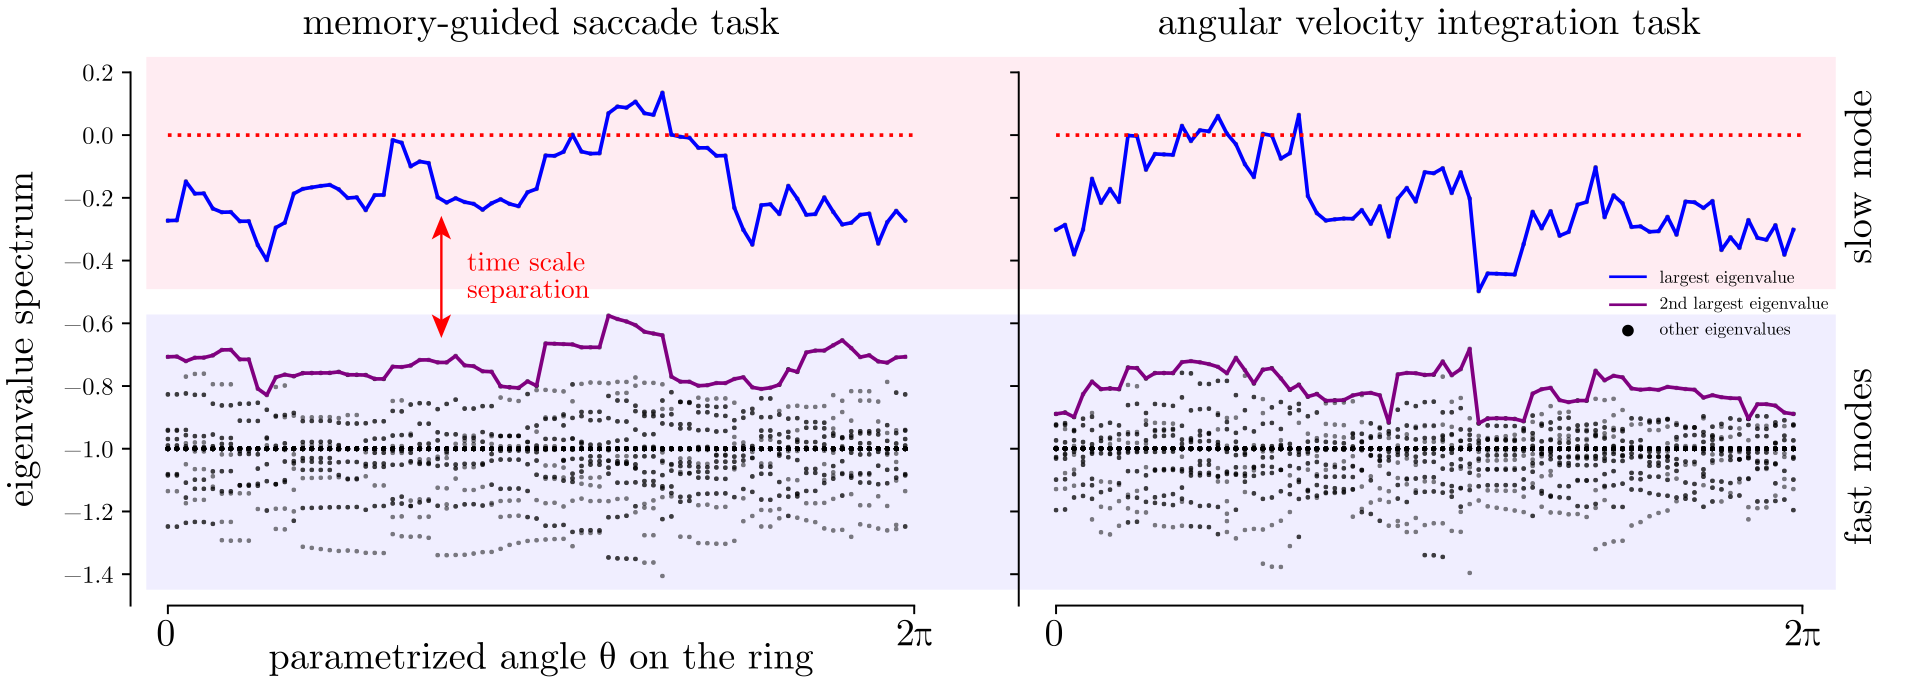
\includegraphics[width=0.8\textwidth]{eigenvalue_gap}
  \caption{The eigenvalue spectrum on invariant manifold show a gap between the first two largest eigenvalues.
    \textbf{(A)} Network trained on the memory-guided saccade task (Fig.4B in the main text).
    \textbf{(B)} Network trained on the angular velocity integration task (Fig.4C in the main text).
}\label{fig:eigenvalue_gap}
\end{figure}


\begin{figure}[tbhp]
  \centering
  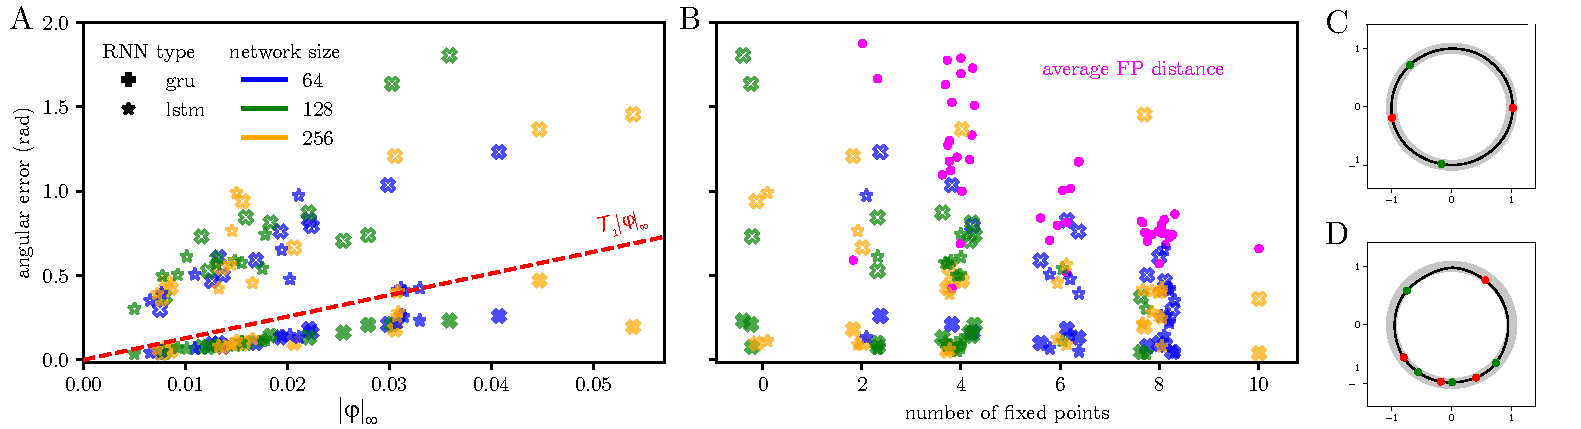
\includegraphics[width=\textwidth]{angular_losses_lstm_gru}
  \caption{The different measures for memory capacity reflect the generalization properties implied by the topology of the found solution.
    \textbf{(A)} The average accumulated angular error vs. the uniform norm on the vector field shown.
     Angular error at \(T_1 =\) trial length (filled markers) and \(\lim T_{1} \to \infty\)  (hollow markers).
      % The number of fixed point is an integer number.
      Points are jittered to aid legibility.
    \textbf{(B)}  The \# of fixed points vs. average accumulated angular error, with the average distance between neighboring fixed points (magenta).
}\label{fig:angular_losses_lstm_gru}
\end{figure}
%A==A
%B==C in main text


\begin{figure}[tbhp]
  \centering
  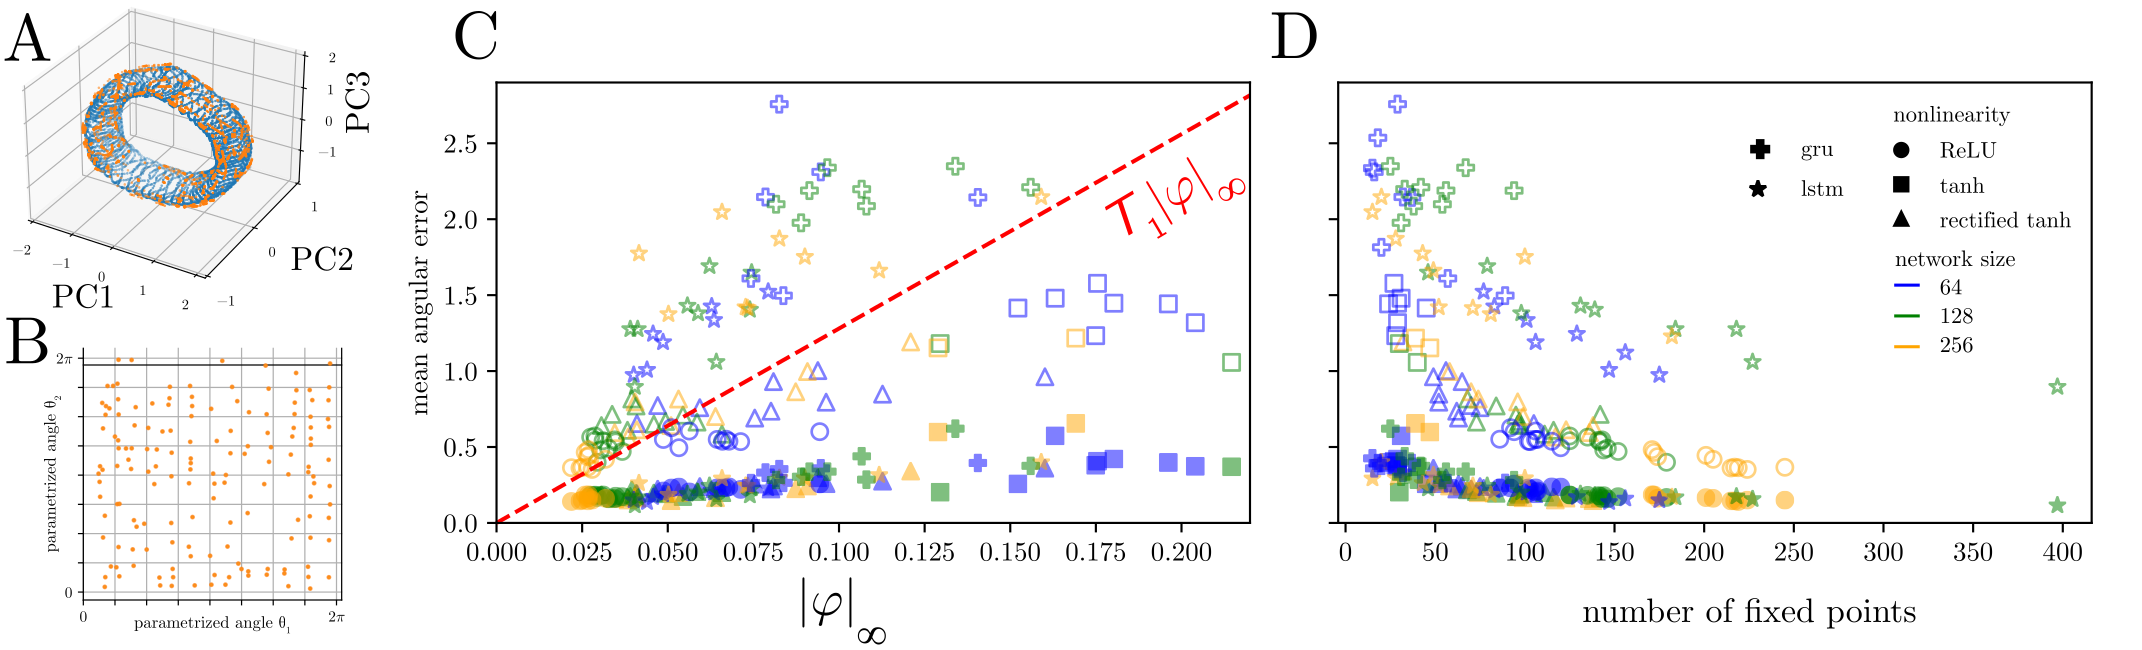
\includegraphics[width=0.8\textwidth]{davit}
  \caption{Networks trained on a double angular velocity integration task.
    \textbf{(A)} Initializations and fixed points of an example network.
    \textbf{(B)} Fixed points on a 2D parametrization of the torus for the example network.
    \textbf{(C)}
    \textbf{(D)}
}\label{fig:davit}
\end{figure}

\end{document}
